\documentclass[10pt,twocolumn]{article}
\usepackage[margin=0.75in]{geometry}
\usepackage[T1]{fontenc}
\usepackage{lmodern}
\usepackage{amsmath,amssymb,booktabs,array,tabularx,graphicx,xcolor}
\usepackage[hyphens]{url}
\usepackage[hidelinks]{hyperref}
\usepackage[numbers,sort&compress]{natbib}
\setlength{\columnsep}{0.25in}
\raggedbottom
\newcolumntype{Y}{>{\raggedright\arraybackslash}X}
\newcommand{\pending}{\textcolor{gray}{Not measured}}
\newcommand{\todo}[1]{\par\noindent\textcolor{blue}{\textbf{Data pending:} #1}\par}
\newcommand{\resultfigure}[4]{%
  \begin{figure}[t]\centering
  \IfFileExists{../figures/#1}{\includegraphics[width=\linewidth]{../figures/#1}}{%
    \fbox{\parbox[c][0.64in][c]{0.92\linewidth}{\centering\small #2\\[3pt]\textcolor{gray}{Measurement not yet available}}}}
  \caption{#3}\label{#4}\end{figure}}

\title{MoE Expert Formats on a Blackwell SM120 GPU:\\A Preliminary Kernel and Energy Characterization}
\author{Author information pending}
\date{Working draft --- 16 October 2026}

\begin{document}
\maketitle

\begin{abstract}
Low-bit expert weights can reduce memory traffic, but the numeric format alone
does not determine executed arithmetic or serving efficiency. We report an
initial 56-point BF16/FP8 W8A8 sweep of single fused MoE layers on one RTX PRO
6000 Blackwell Server Edition GPU (SM120). Synthetic weights and routing use
OLMoE and Qwen3-30B-A3B layer shapes, an explicitly selected Triton path, and
untuned fallback configurations. FP8 has lower median latency at all 28
matched loads: BF16/FP8 latency ratios are 1.14--1.86 for OLMoE and 1.16--1.92
for Qwen3. An additional 14-point calibrated Qwen3 first-layer NVFP4/CUTLASS
sweep shows a nonmonotonic relative ranking: NVFP4 is faster at sampled
$B=8$ through 2048, while FP8 is faster at $B=1$ and 8192, for both routing
distributions. The comparison matches shape, routing and graph mode, but
uses different weight sources and untuned paths. It establishes neither a
switching threshold nor quality or serving benefits. Original BF16/FP8
energy windows include restart from idle; NVFP4 uses a revised continuous-load
warmup protocol and is reported separately. Fourteen calibrated AWQ points
complete the 56-point Qwen3 four-format grid: AWQ has the lowest median at
$B=8,32,128,512$, NVFP4 at 2048, and FP8 at both endpoints, for both
routing distributions. The lowest-latency path need not have the lowest
device energy. Static SM120 SASS distinguishes Marlin BF16 arithmetic from
CUTLASS FP4 arithmetic, subject to the recorded binary-identity limits.
Dual-format serving remains unmeasured. Prior runtime precision
adaptation motivates a characterization, rather than a first-switching claim.
\end{abstract}

\section{Introduction}
MoE execution combines a large resident weight set with an input-dependent
number of tokens per expert. A format that minimizes transferred weight bytes
may incur additional scale handling, dequantization, padding, or dispatch
cost. Conversely, a compute-efficient path may not amortize its overhead at
small expert batches. These observations motivate measuring implemented
format paths over the expert loads that a serving workload actually produces.

The planned scope is two model architectures, OLMoE and Qwen3-30B-A3B, on a
single SM120 GPU using vLLM 0.26.0. The main question is whether format rankings
change across this scope and whether such changes survive full serving costs,
quality checks, and equal total-memory budgets. A crossover is a hypothesis,
not an assumption needed to make the study useful.

Runtime precision adaptation is established prior work. DynaExq changes
expert precision using online routing history under a memory cap
\citep{dynaexq}; PagedWeight changes precision in response to KV-cache pressure
\citep{pagedweight}. We therefore do not claim the first workload-aware
expert-precision switch. The proposed contribution is a measured account of
SM120 format behavior and its practical decision boundaries. A simple
dual-format policy remains an implementation and evaluation subject.

The completed evidence covers synthetic single-layer BF16/FP8 execution,
a calibrated Qwen3 first-layer NVFP4 load curve, and a complete AWQ
native-Marlin load curve with execution evidence. The fastest of these four
paths changes three times between sampled loads, challenging a single
monotonic selection threshold. Workload-derived loads, quality evaluation, and serving costs
remain unresolved. Different weight sources prevent treating these kernel
comparisons as an interchangeable same-model policy evaluation.

\section{Background and Scope}
For a routed SwiGLU expert, input width $d$ and intermediate width $h$ define
gate, up, and down projections. With $E$ experts and top-$k$ routing, a step
with $B$ input tokens has $Bk$ token--expert assignments. The uniform average
$Bk/E$ is not the load of every expert. We retain the vector
$\mathbf{M}=(M_1,\ldots,M_E)$ and distinguish workload traces from constructed
uniform and skewed diagnostic cases.

We distinguish storage format, activation format, scale granularity, and
the executed kernel. An NVFP4 checkpoint does not prove FP4 tensor-core
execution. vLLM's versioned NVFP4 selector exposes several backends and warns
of shape-specific fallbacks \citep{nvfp4oracle}. Its SM12x FlashInfer integration
requires explicit selection in this release, and availability of that source
path is not evidence that it ran correctly on our machine \citep{b12x}.
ModelOpt supplies quantized model artifacts, while vLLM selects the execution
path \citep{modelopt,vllmmodelopt}.

\section{Characterization}
\subsection{Platform and measurements}
The measured platform is one RTX PRO 6000 Blackwell Server Edition (SM120),
with driver 580.95.05, vLLM 0.26.0, PyTorch 2.11.0+cu130, CUDA 13.0, and
Triton 3.6.0. The installed FlashInfer package is 0.6.14, but the completed
sweep explicitly invokes vLLM's Triton \texttt{fused\_experts} entry point;
it does not use automatic backend selection. All eight model/format/routing
arms report missing device-specific configuration files and use default MoE
configurations. The additional Qwen3 NVFP4 sweep explicitly selects CUTLASS.
These are untuned path comparisons, not best-backend comparisons.

CUDA events measure graph replay after ten warmup calls. Five trials per
point each contain repeated invocations; the median and full min--max range
are retained. These are repetitions within one process, not independent
system runs or confidence intervals. Inputs, weights, and routing are fixed
within each point, with no cache flush. The boundary includes expert
alignment/permutation, both projections, SiLU, and output summation; FP8
also includes activation quantization. Precomputed top-$k$ assignments are
supplied, so router selection is excluded. Compilation and initialization
are outside this steady replay latency measurement. A separate profiler call
records the underlying kernels.

All 56 original energy points use differences of the NVML total-energy counter as
the primary measurement. Power is additionally polled every 50 ms for a
diagnostic integral. Total and idle-subtracted window energies are retained:
\begin{align}
 E_{\rm total}&=\int_{t_0}^{t_1}P(t)\,dt,\\
 E_{\rm incremental}&=E_{\rm total}-P_{\rm idle}(t_1-t_0).
\end{align}
Here the integral denotes the physical quantity; the plotted total is
measured by the counter. The original windows last 3.001--3.022 s and start
when load resumes after an idle-baseline interval. They therefore include
the load transition and are not steady-state energy estimates. Each plotted
value is divided by the number of completed layer invocations times their
input tokens. There is one energy window per point and no repeated-window
error bar. This denominator is \emph{single MoE-layer input tokens}, not
generated tokens. Raw counters, samples, duration, and both energy estimates
are preserved.

The sampled integral is 9.30--17.71\% below the counter in the original sweep.
NVML documents that \texttt{nvmlDeviceGetPowerUsage} returns one-second
averaged power on Ampere, except GA100, and newer GPUs \citep{nvmlpower};
50-ms polling does not provide 50-ms physical resolution. A follow-up at one
synthetic uniform FP8 point ($B=512$, OLMoE shape) records signed
sample/counter differences of $-18.92\%$ after idle, then $+1.38\%$ and
$+0.19\%$ in two successive loaded windows. This supports a load-transition
lag explanation at that point; it does not validate all original windows
as steady state or establish the cause of every discrepancy. Subsequent
energy measurements resume load for three seconds after the idle baseline
before opening the counter window. The NVFP4 sweep below uses this revised
protocol (v2); original F2 data are retained without mixing the protocols.

\begin{table*}[t]
\centering\small
\caption{T1: Execution evidence on SM120. BF16/FP8 have profiler and compiled
JIT PTX evidence. NVFP4 and AWQ each have 14 calibrated first-layer points,
numerical diagnostics, and profiler names matched to static SM120 SASS
functions. The NVFP4 historical trace did not record a library hash;
its match is to the currently installed binary. Static instructions are
not dynamic hardware instruction counts.}
\label{tab:paths}
\begin{tabularx}{\textwidth}{lYYYY}
\toprule
Format & Observed path / status & Activation / scaling & Arithmetic evidence & Evidence boundary \\
\midrule
BF16 & Triton; \texttt{fused\_moe\_kernel} & BF16; no quantization scales &
\texttt{mma.sync}, \texttt{m16n8k16}, BF16 inputs, FP32 accumulation &
28 points; profiler plus cached JIT PTX \\
FP8 W8A8 & Triton; \texttt{fused\_moe\_kernel} plus dynamic FP8 quantization &
E4M3; per-expert tensor weight scales, dynamic tensor activation scales &
\texttt{mma.sync}, \texttt{m16n8k32}, E4M3 inputs, FP32 accumulation &
28 points; profiler plus cached JIT PTX \\
NVFP4 & CUTLASS; calibrated Qwen3 layer 0 executes &
W4A4; block-16 scales and calibrated per-expert global scales; BF16 input/output &
Matched current SM120 SASS: \texttt{OMMA.SF}, E2M1 inputs, FP32 accumulation &
14 points; historical library identity not independently established \\
AWQ W4A16 & Native Marlin; calibrated Qwen3 layer 0 executes &
Symmetric INT4, group-128 weight scales; BF16 activations &
Matched SM120 SASS: \texttt{HMMA.16816}, \texttt{F32.BF16} &
14 points; static instruction evidence tied to one $B=1$ profiler specialization \\
\bottomrule
\end{tabularx}
\end{table*}

\paragraph{Calibrated NVFP4 smoke.}
The first expert layer of \texttt{nvidia/Qwen3-30B-A3B-NVFP4}, revision
\texttt{2538ded2a4ed}\ldots, is converted through vLLM's native CUTLASS
layout path. The publisher does not report the exact base-model revision;
the quantized revision and tensor hashes are retained with the artifact.
At $B=8$ with constructed uniform assignments, the layer executes with
finite output. The profiler records a CUTLASS kernel whose symbol contains
\texttt{MainloopSm120ArrayTma}\allowbreak\texttt{WarpSpecializedBlockScaled}
and \texttt{float\_e2m1\_t}. Five eager CUDA-event repetitions give a
median of 0.1978523 ms. This smoke uses pretrained calibrated weights and
eager timing, so its latency is not directly compared with the synthetic
graph-replay curves in F1.

A separate two-token constructed-input check examines 15 selected experts:
source-to-processed weight order, block scales, and fused scale relations
all pass. An independent E2M1 decoder and FP32 matrix multiplications, with
TF32 disabled and BF16-rounded SiLU product before activation quantization,
give relative $L_2$ error 0.01646 and cosine similarity 0.999866 against the
CUTLASS output. This is a layout/scale and numerical integration diagnostic,
not an lm-eval result or a model-quality guarantee.

The archived $B=1$ CUTLASS profiler symbol exactly matches a single
SM120 function in the currently installed
\texttt{\_C\_stable\_libtorch.abi3.so}. Its disassembly contains 64 static
\texttt{OMMA.SF.16864.F32.}\allowbreak\texttt{E2M1.E2M1.UE4M3.4X}
instructions. NVIDIA identifies \texttt{OMMA} as FP4 matrix multiply and
accumulate across a warp.\footnote{NVIDIA CUDA Binary Utilities 13.0.3,
Blackwell instruction set:
\url{https://docs.nvidia.com/cuda/archive/13.0.3/cuda-binary-utilities/index.html\#blackwell-instruction-set}.}
The original trace did not record the library hash, so the symbol match
does not independently prove historical binary identity. This static
match supports path classification, not dynamic execution counts.

\paragraph{Calibrated AWQ execution diagnostic.}
The first expert layer from \texttt{dtometzki/Qwen3-30B-A3B-awq-sym},
revision \texttt{c3b14f75be5e}\ldots, is converted by vLLM's native
WNA16/Marlin path as symmetric INT4 (\texttt{uint4b8}), with group-128
scales and BF16 activations. The publisher documents AWQ calibration;
its exact base-model revision is unreported. In
\texttt{qwen3\_awq\_export\_r02}, native Marlin produces finite output for
two constructed tokens selecting 15 experts. An independent signed-INT4
decode of source tensors and FP32 reference gives relative $L_2$ error
0.004361 and cosine similarity 0.999991; a swapped gate/up negative control
has relative $L_2$ error 0.5656. This supports the tested conversion and
execution wiring, without a task-quality claim. The processed artifact and
diagnostic are locally hash-verified. All 14 uniform/Zipf graph-replay points
now have latency, energy, and profiler records.
For the $B=1$ trace, the demangled Marlin kernel name exactly matches the
unique selected function in the library's SM120 SASS dump; that function
contains \texttt{HMMA.16816.}\allowbreak\texttt{F32.BF16} instructions.
The source-library hash, symbol, command and disassembly are retained in
\path{runs/awq_compiled_paths/}. This ties static arithmetic evidence to an
actually observed specialization, not to dynamic instruction counts or
every Marlin specialization in the sweep.

\subsection{Load, latency, and energy curves}
The completed run, \texttt{twoformat\_survey\_r01}, contains all 56 planned
points: two layer shapes, two formats, uniform/Zipf synthetic routing, and
$B\in\{1,8,32,128,512,2048,8192\}$. Both shapes use $d=2048$ and top-$k=8$;
OLMoE uses $(h,E)=(1024,64)$ and Qwen3 uses $(768,128)$. Weights are synthetic
Gaussian values; FP8 weights are quantized from them. These are architecture
shapes, not full models with pretrained weights. Workload-derived routing
histograms have not yet been measured.

Figure~\ref{fig:latency} plots the mean assignment count $Bk/E$, including
inactive experts. FP8 has lower median latency at all 28 matched points.
The BF16/FP8 ratios span 1.14--1.86 for OLMoE and 1.16--1.92 for Qwen3.
Thus there is no sampled BF16/FP8 latency crossover in this particular
untuned Triton sweep; connecting adjacent observations is not a fitted
crossover estimate. The result supports a fixed FP8 latency choice within
this tested synthetic domain. It does not show that tuning or another
backend could not change the ranking, and does not address FP8 versus 4-bit.

Figure~\ref{fig:energy} reports the original restart-window measurements.
FP8's recorded total-counter joules per input token are lower at all matched
points (27.9--49.0\% lower across the two shapes), but these percentages
describe those finite windows only. They do not establish steady-state
energy savings, model-level energy per generated token, or a quality-aware
format recommendation. The single-point sensor diagnostic motivates
separate steady-load confirmation before making such claims.

\paragraph{Qwen3 NVFP4 load sweep.}
The completed \texttt{qwen3\_nvfp4\_survey\_r02} adds 14 points at the same
seven $B$ values and two synthetic routing distributions. All produce finite
outputs and matching eager/graph outputs. Figure~\ref{fig:qwen-four}
compares the calibrated NVFP4 first layer with the earlier synthetic
BF16/FP8 weights. Layer shape, routing histograms, and graph-replay timing
match; weight provenance and backend do not. The figure therefore compares
these executed paths, not the effect of format alone on identical weights.

For both routing distributions, NVFP4 has lower median latency at sampled
$B\in\{8,32,128,512,2048\}$; the FP8/NVFP4 ratios are 1.094--1.461 for
uniform and 1.150--1.414 for Zipf routing. FP8 is faster at $B=1$ and 8192.
This U-shaped \emph{relative ordering} is not a U-shaped absolute latency
curve. Rank changes are only bracketed by the adjacent observations
$[1,8]$ and $[2048,8192]$. We do not interpolate crossings or fit a
threshold $\theta$. Five within-process timing repetitions do not provide
independent run-level uncertainty or validate an online selector.

\paragraph{Complete sampled four-format grid.}
The same figure includes 14 calibrated AWQ points, completing all 56
Qwen3 format/routing/load combinations. In both routing distributions,
FP8 has the lowest median at $B=1,8192$, AWQ at $B=8,32,128,512$, and
NVFP4 at $B=2048$. AWQ's FP8/AWQ ratios at its four winning loads are
1.704--2.211 for uniform and 1.492--3.449 for Zipf routing. The observed
winner changes are bracketed by $[1,8]$, $[512,2048]$, and $[2048,8192]$;
these are neither fitted crossing points nor deployed thresholds. Some
adjacent differences are small: at uniform $B=2048$, AWQ/NVFP4 is 1.027,
and at uniform $B=8192$, NVFP4/BF16 is 1.011. Within-process repeat ranges
do not establish independent-run significance. The public low-bit
checkpoints have distinct provenance; this remains an untuned path
comparison, not a same-weight quality comparison.

The original AWQ $B=2048$ run failed a bitwise graph/eager comparison.
Follow-up repeats also differ within eager mode. The nine remaining points
were therefore measured under an explicitly revised acceptance rule:
finite outputs, relative $L_2\leq\epsilon_{\rm BF16}/8$, and maximum
absolute error $\leq\epsilon_{\rm BF16}\max|y_{\rm reference}|$.
Three accepted cases are not bitwise equal (uniform $B=2048,8192$ and Zipf
$B=8192$); their largest relative $L_2$ and absolute differences are
$2.3012\times10^{-5}$ and 0.001953125. The old failure and all revised checks
remain in the summary. This capture-consistency check is not model-quality
validation, and we do not attribute the differences to unverified atomics.

\paragraph{Instrumented component accounting.}
Figure~\ref{fig:qwen-components} separates the existing profiler traces at
$B\in\{1,8,2048,8192\}$ into whole projection kernels, activation and
quantization, row shuffles, output operations, and setup/other kernels.
Every bar is one instrumented graph replay. Its height is the sum of GPU
kernel durations, not the five-trial unprofiled latency median, and not a
wall-clock interval: inter-kernel gaps and any overlaps are not adjusted.
The profile-sum ordering matches the unprofiled median ordering at these
eight selected routing/load cases, but their numerical magnitudes should
not be interchanged. No independent-run uncertainty is available for this
component view.

At $B=1$, NVFP4 has both longer projection kernels and more time outside
those kernels than FP8. At $B=8$ and 2048, its projection-time reduction
exceeds its additional non-projection time. At $B=8192$, that balance
reverses: NVFP4 projection kernels sum to 0.706 versus 1.163 ms for uniform
routing, and 0.804 versus 1.349 ms for Zipf routing. However, its remaining
kernels sum to 1.682 and 1.670 ms, versus FP8's 0.646 and 0.636 ms.
NVFP4 row shuffles alone account for 0.520/0.532 ms and output operations
for 0.652/0.649 ms (uniform/Zipf). Thus an additional 1.036/1.034 ms outside
the projection kernels outweighs their 0.457/0.545 ms reduction in these
instrumented replays.

An additional 12-trace comparison at $B=2048,8192$ adds AWQ to these
two paths, preserving the eight reused FP8/NVFP4 component sums exactly.
At $B=8192$, AWQ's complete Marlin projection kernels take 2.078/2.217 ms
(uniform/Zipf), or 82.87/83.39\% of its summed kernel time. FP8's projections
take 1.163/1.349 ms. AWQ's remaining kernels are shorter than FP8's by
216.672/194.273 $\mu$s, but this does not offset its longer projections.
Thus AWQ's high-load loss is located inside the projection kernels,
whereas NVFP4's is located outside them. At $B=2048$, AWQ's projection
excess is only 21.637/37.790 $\mu$s and its other kernels save
48.638/49.633 $\mu$s; the summed time and unprofiled median both remain
below FP8's. Each trace contains one instrumented graph replay, so these
differences are an observed decomposition, not an independent repeat
estimate or an achievable optimization gain.

This accounting identifies where the recorded kernel-duration difference
appears; it does not isolate the causal cost of equivalent primitives.
Projection kernels fuse different work across the three backends, and the
auxiliary groups consequently have different boundaries. The comparison
also retains synthetic FP8 weights versus distinct calibrated AWQ/NVFP4
weights. Without dynamic hardware counters or a controlled intervention,
these traces establish neither pure tensor-core efficiency, a
dequantization or bandwidth bottleneck, nor a counterfactual fusion benefit.

Figure~\ref{fig:qwen-energy} reports 14 NVFP4 and 14 AWQ energy points
under protocol v2.
After the per-point idle baseline, three seconds of continuous workload
precede each approximately three-second counter window (2.982--3.037 s).
The signed difference $100(E_{\rm sampled}/E_{\rm counter}-1)$ ranges
from $-0.546\%$ to $+3.000\%$ for the 14 NVFP4 points and
$-3.994\%$ to $+0.631\%$ for the 14 AWQ points; the median across all
28 is $+0.075\%$.
Agreement between the two measurement methods is a local diagnostic, not a repeated-run
uncertainty estimate. Total and idle-subtracted device energy are divided
by completed single-layer input tokens. We do not compare these v2 values
against the original BF16/FP8 restart windows or infer model-level energy
per generated token. AWQ/NVFP4 total-energy ratios range from 0.610 to
1.322 for uniform routing and 0.473 to 1.385 for Zipf; idle-subtracted
ratios are 0.604--1.398 and 0.512--1.455. The total-energy ordering reverses
between $B=512$ and 2048 for uniform routing, but between 128 and 512 for
Zipf. Idle subtraction moves the uniform reversal to $[128,512]$.
At Zipf $B=512$, the NVFP4/AWQ latency ratio is 1.108, but AWQ uses
14.27\% more total and 21.61\% more idle-subtracted energy. At uniform
$B=512$, AWQ's total energy is 3.88\% lower and its incremental energy
1.08\% higher. These single-window observations separate latency and
energy objectives; especially small gaps require independent repetition.

\begin{figure*}[t]
\centering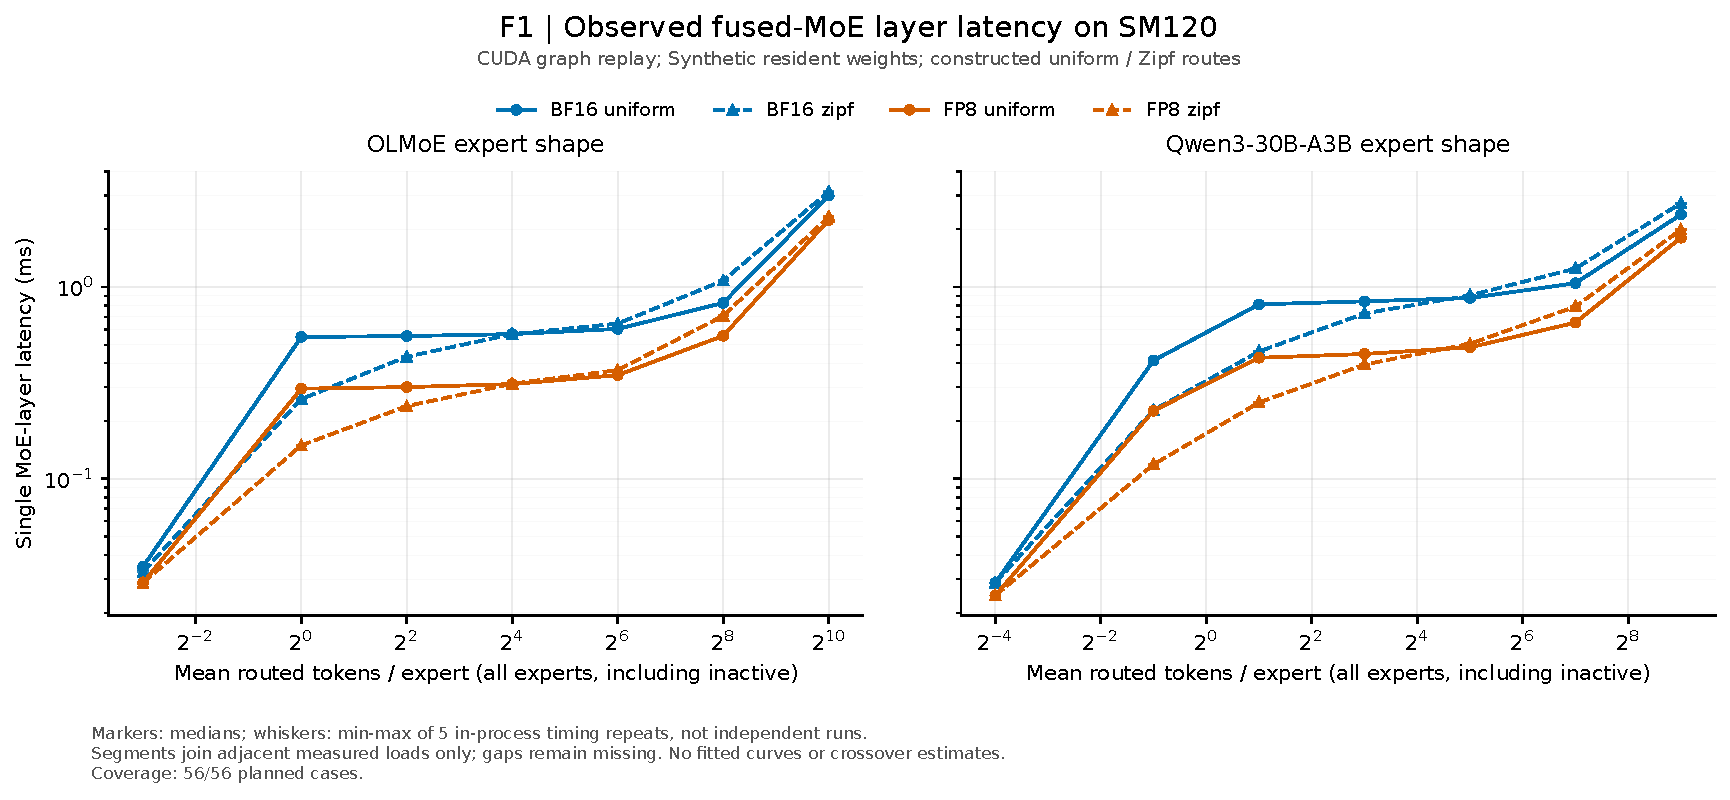
\includegraphics[width=\textwidth]{../figures/F1_latency.pdf}
\caption{F1: Measured single-layer graph-replay latency, synthetic weights
and routing, explicit Triton backend with default configurations. The
horizontal axis includes inactive experts. Lines connect observations;
whiskers show min--max over five repetitions within one process, not independent
run uncertainty. No sampled BF16/FP8 crossover is observed.}
\label{fig:latency}
\end{figure*}
\begin{figure*}[t]
\centering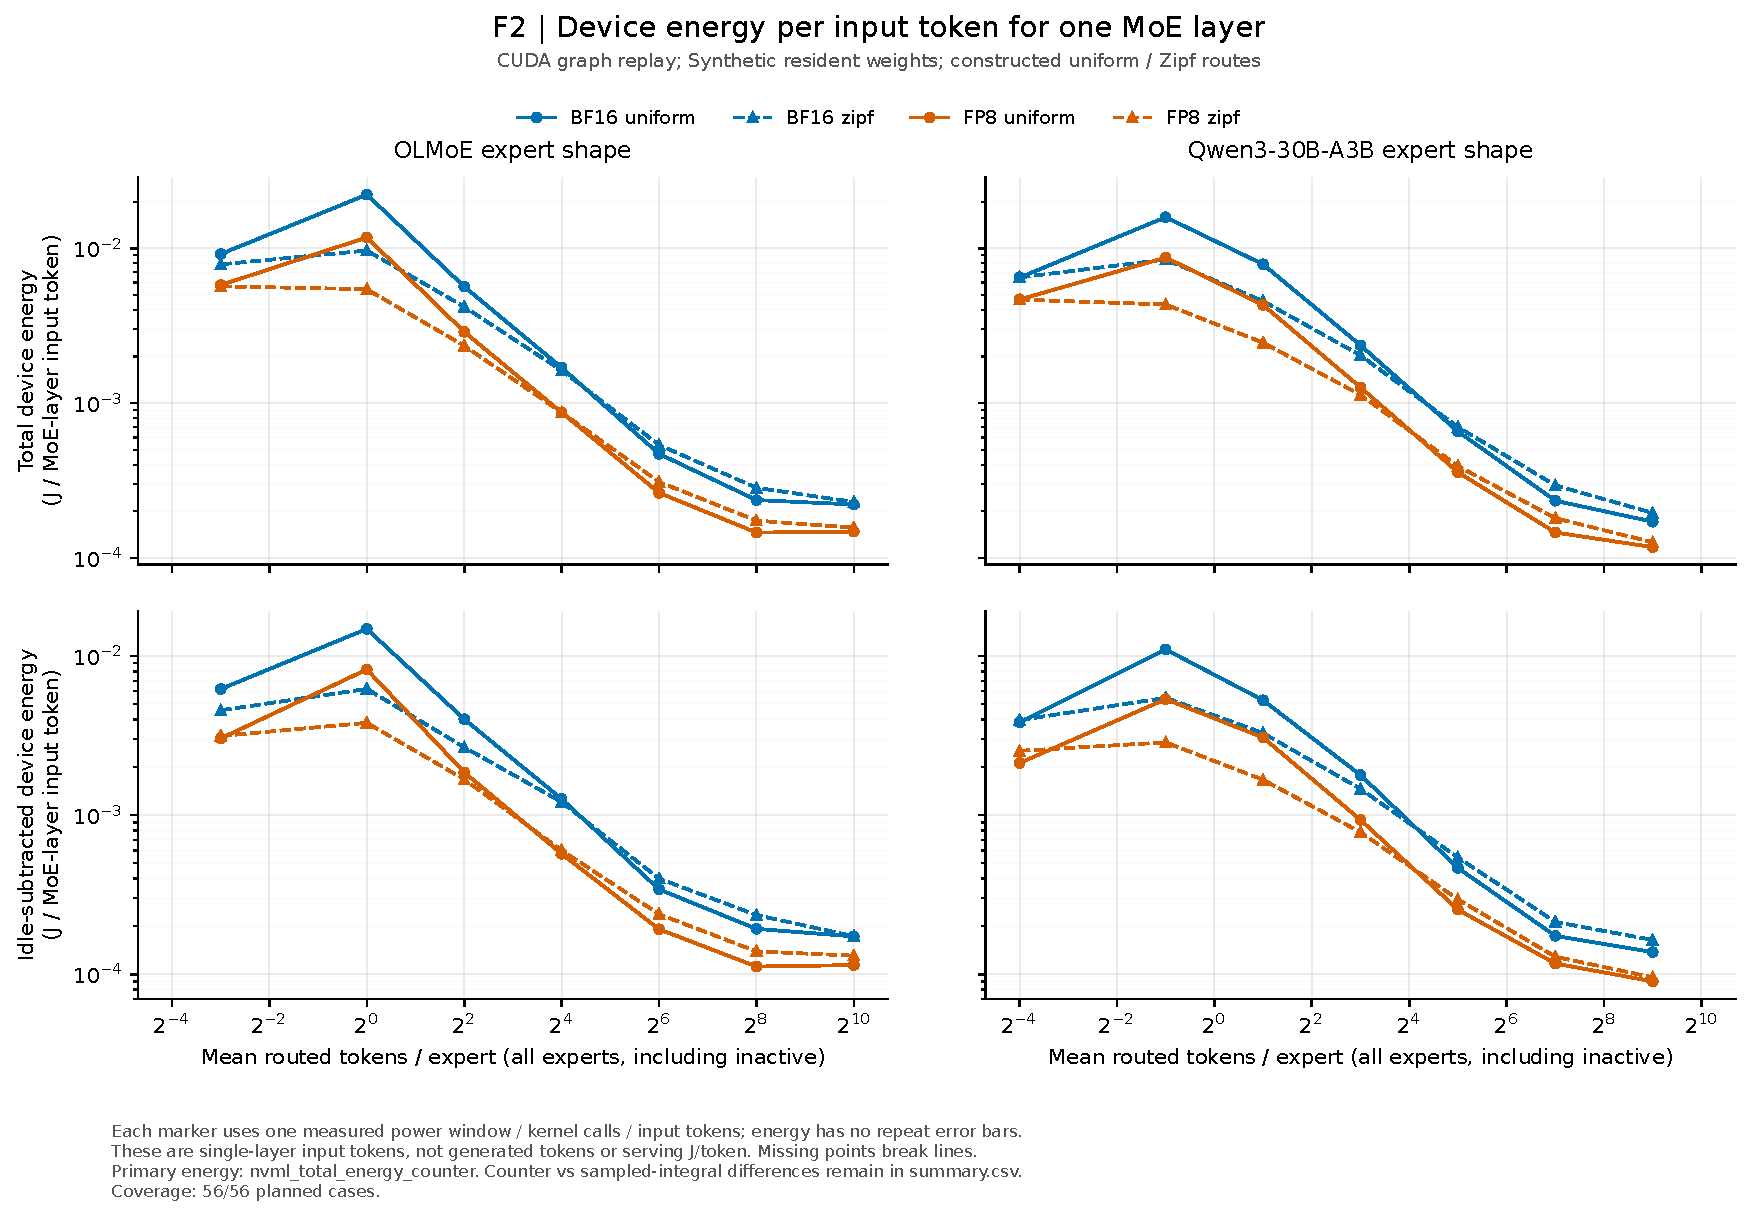
\includegraphics[width=\textwidth]{../figures/F2_energy.pdf}
\caption{F2: Original approximately three-second \emph{restart} windows,
including resumption from idle, measured by the NVML total-energy counter.
Top: total energy. Bottom: idle-subtracted energy. Both use single MoE-layer
input tokens as denominator. One window per point; no energy error bars.
These curves are not steady-state or serving energy estimates.}
\label{fig:energy}
\end{figure*}
\begin{figure*}[t]
\centering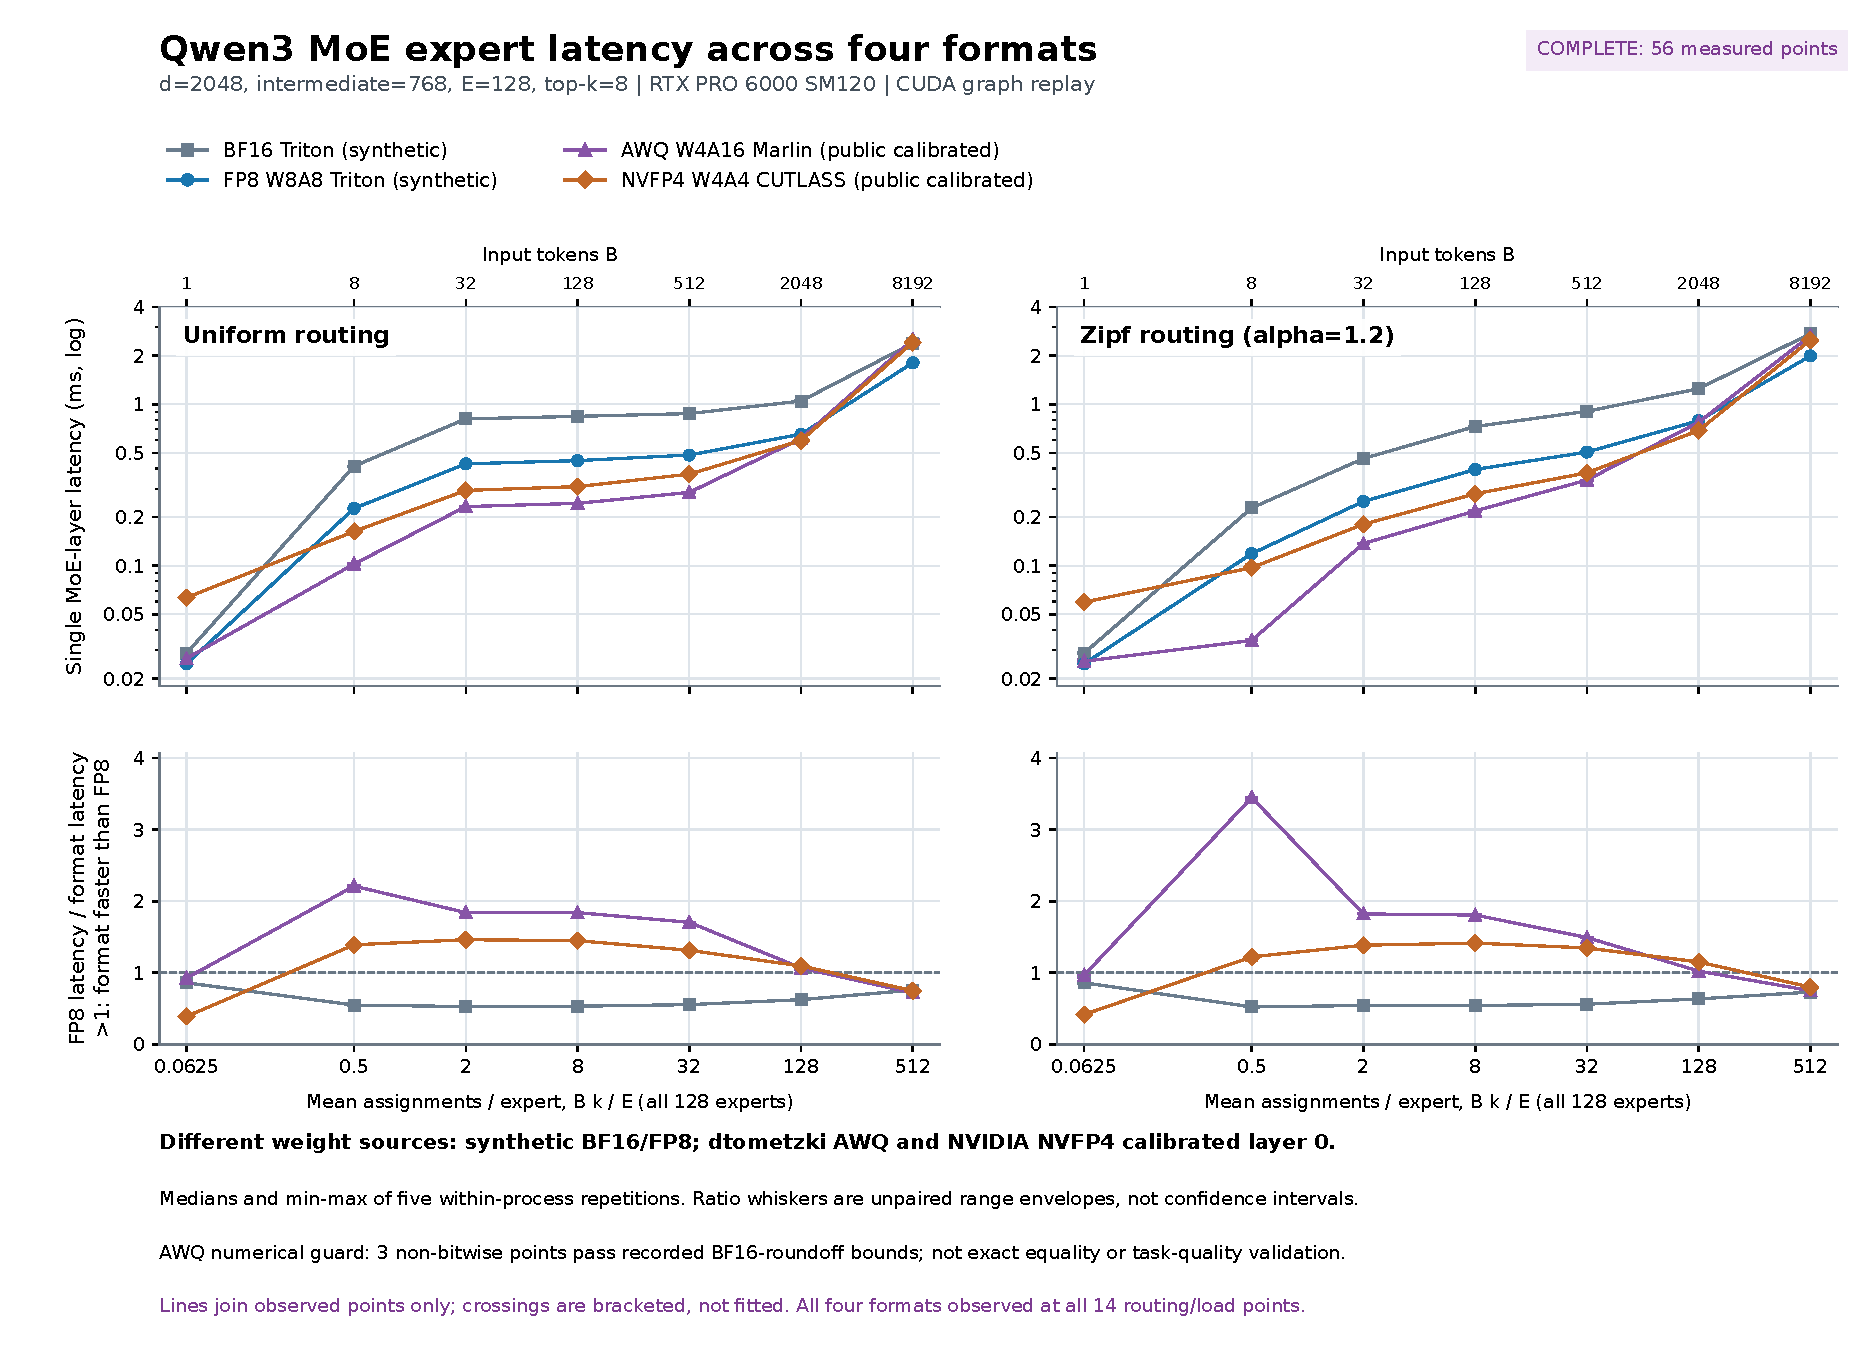
\includegraphics[width=\textwidth]{../figures/F1_qwen_four_formats.pdf}
\caption{F1 extension: Complete 56-point Qwen3-shape four-format graph-replay latency
grid. BF16/FP8 use synthetic weights and Triton; AWQ/Marlin
and NVFP4/CUTLASS use distinct calibrated first-layer checkpoints. Routing
histograms match. Markers are medians; whiskers are five within-process
repetitions. Three AWQ cases pass the declared BF16-roundoff check without
bitwise graph/eager equality. Rank-change brackets are not fitted thresholds.}
\label{fig:qwen-four}
\end{figure*}
\begin{figure*}[t]
\centering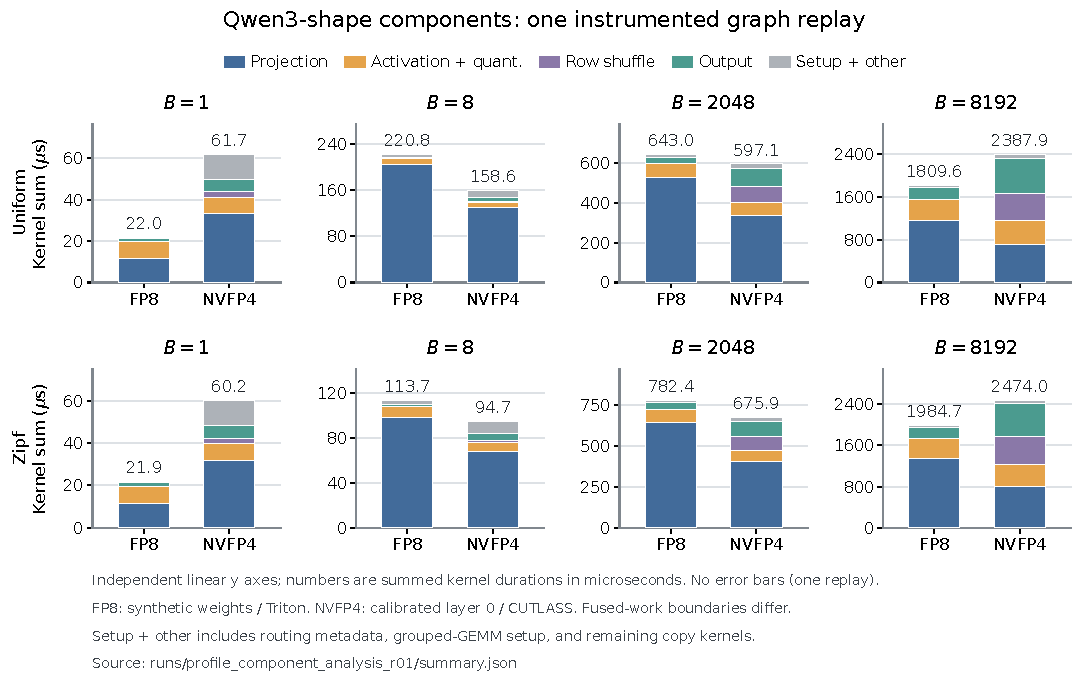
\includegraphics[width=\textwidth]{../figures/F1b_qwen_components.pdf}
\caption{F1b: Qwen3-shape component accounting from
\protect\path{runs/profile_component_analysis_r01/summary.json}.
Rows show uniform and Zipf routing; columns show input-token counts
$B=1,8,2048,8192$. Each panel has an independent linear y-axis in
microseconds; numbers above bars are summed GPU kernel durations.
Each bar is one instrumented CUDA-graph replay, so no error bars are drawn.
Setup/other includes routing metadata, grouped-GEMM setup, and remaining
copy kernels. FP8 uses synthetic weights and Triton; NVFP4 uses a calibrated
Qwen3 first layer and CUTLASS. Different fused-work boundaries and weight
sources preclude a same-weight format-only or causal fusion comparison.
These sums do not replace the unprofiled latency medians.}
\label{fig:qwen-components}
\end{figure*}
\begin{figure*}[t]
\centering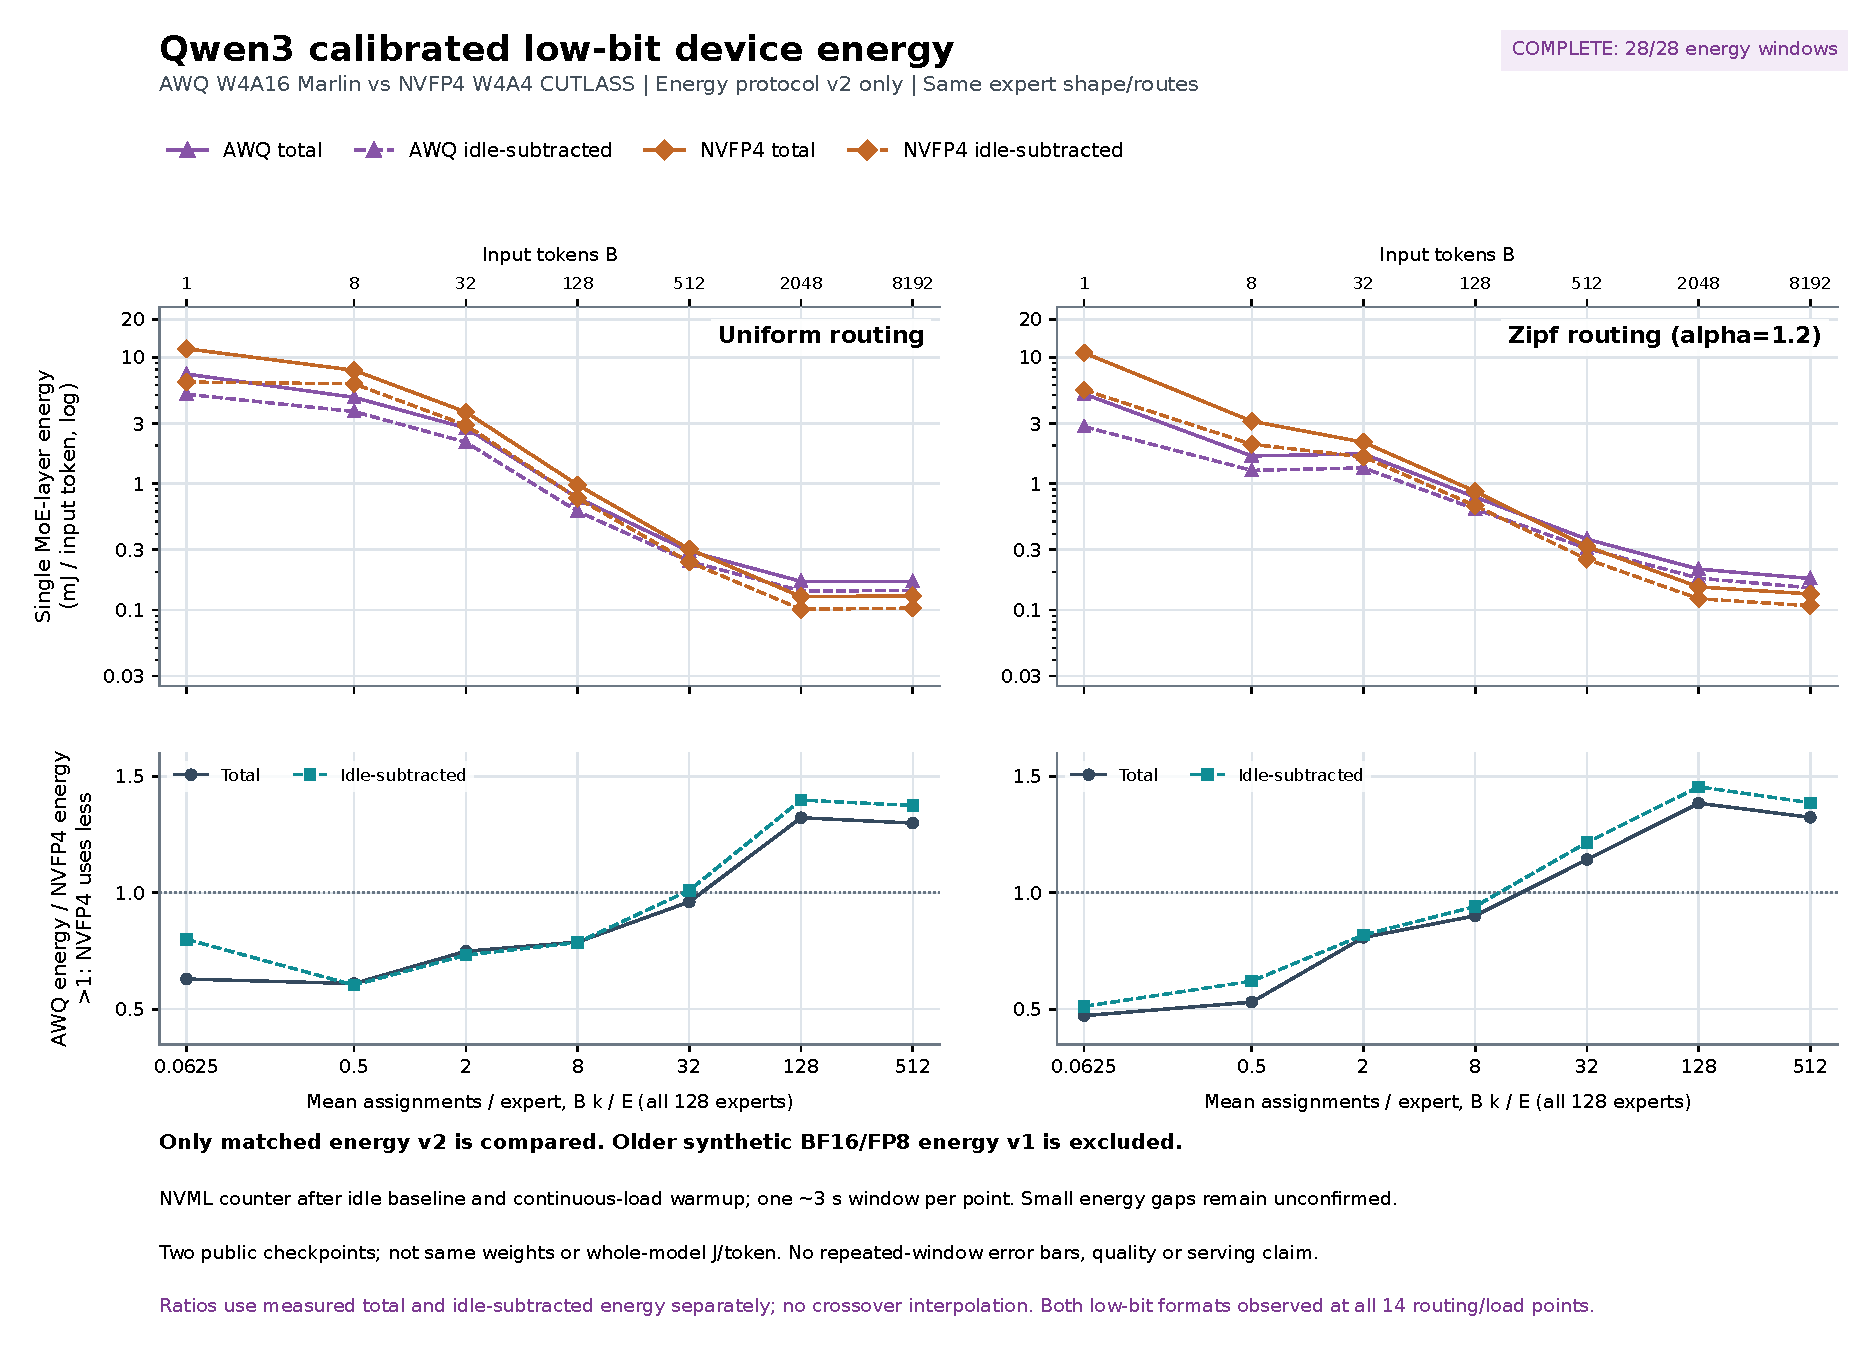
\includegraphics[width=\textwidth]{../figures/F2_qwen_awq_nvfp4_energy_v2.pdf}
\caption{F2 extension: 14 NVFP4 and 14 AWQ device-energy points under protocol v2, with
continuous-load warmup after idle. Units in the plot are millijoules per
single MoE-layer input token. One counter window per point; total and
idle-subtracted values have no repeated-window uncertainty estimate. The
bottom row shows AWQ/NVFP4 ratios; the unit line marks equal measured energy.
Earlier BF16/FP8 energy protocol v1 is excluded from comparison.}
\label{fig:qwen-energy}
\end{figure*}

\section{Model and Simple Format Selection}
An explanatory approximation for a single expert is
\begin{equation}
 T_f(M_e)\approx
 \max\left\{\frac{6dhM_e}{C_f},\frac{3dhb_f}{W_f}\right\}+c_f,
\end{equation}
where $b_f$ is stored bytes per weight, $C_f$ and $W_f$ are effective rates,
and $c_f$ represents fixed overhead. Scale bytes, activation traffic,
nonlinearities, and grouped-kernel interaction require explicit accounting
when material. This approximation is neither a hardware peak prediction nor
a validated upper bound. Effective crossover points are read from measured
curves rather than inferred from nominal bit widths.

For fused execution, the empirically relevant quantities are
$T_f(\mathbf{M})$ and $E_f(\mathbf{M})$; generally,
$T_f(\mathbf{M})\ne\sum_eT_f(M_e)$ because experts share GPU resources.
A step-level rule chooses FP8 when $\max_eM_e\geq\theta$ and the selected
4-bit path otherwise. The direction of this rule is retained only if data
support it. The measured Qwen3 FP8--NVFP4 ordering now changes twice in $B$,
so a single monotonic threshold is not justified by these curves. No
$\max_e M_e$ threshold is fitted from the two $B$ brackets. Whether a
bounded-load rule has value requires compatible weights, workload-derived
loads, and an executed policy comparison. If one format dominates in that
comparison, the fixed-format result is reported.
The phase baseline chooses FP8 for pure prefill, 4-bit for pure decode, and
uses the same threshold for mixed steps.

The conceptual objective is energy reduction subject to task-quality and
service constraints. A local kernel decision cannot guarantee request-level
P95 TPOT, so feasibility is established by serving measurements, not claimed
from the threshold equation. No online predictor or bandit is introduced.

\section{Implementation}
The artifact-backed prototype in \texttt{code/dual\_format\_moe.py} subclasses
vLLM 0.26.0's \texttt{FusedMoEMethodBase} \citep{vllm026}. It delegates to two
real resident-format backends and checks matching layer shape, weight
provenance, and an activation-basis contract. The routed-experts
runner supplies top-$k$ selection once; the
prototype implements step-threshold and explicit prefill/decode phase rules.
The \texttt{dual\_format\_worker.py} Worker subclass installs the method
after weight loading and before KV sizing and warmup. It verifies each
layer's actual post-attention RMSNorm parameter bytes and epsilon against
the artifacts' basis descriptors and saved norm tensors; a supplied ID
alone cannot pass the check. The worker now derives phase labels from
the scheduler's computed-token positions and prompt boundaries for the
scheduled token spans, including mixed steps, rather than guessing phase
from batch token count. Seven CPU boundary tests pass. The worker hook and
phase dispatch still lack GPU execution validation. This prototype is not
part of either completed curve sweep and has no completed serving-performance
or mixed-generation quality result; it is not a stock serving quantization mode.

Shared checkpoint lineage alone does not establish compatible expert input
coordinates: AWQ smoothing can change preceding normalization, router, and
expert weights. Production installation therefore requires matching explicit
\texttt{activation\_basis\_id} values for both artifacts and the actual
worker layer. The implemented hash verifies the local normalization
transform; it does not certify upstream activation equality or router
quality. Existing
public sidecars without that evidence are rejected by default. There is no
branch-specific input adapter. An explicit mechanism-only override permits
dispatch diagnostics, but establishes neither output semantics nor quality;
matching metadata IDs likewise cannot replace the underlying verification.

The current prototype supports eager single-GPU execution. Its maximum
expert count uses a CPU-visible \texttt{item()} and therefore incurs a device
synchronization; this cost cannot be omitted from a future policy comparison.
Dynamic switching within CUDA graph capture and compiled execution is
rejected. An expert-split code path uses native expert maps for FP8 Triton
and AWQ Marlin, but awaits GPU validation of masking and accumulation.
NVFP4 expert splitting is rejected. The worker code, CPU phase checks, and
basis guard do not establish a validated GPU serving integration.

Two full expert copies consume approximately 1.5 bytes per expert parameter
before scales, metadata, non-expert weights, workspaces, and KV cache.
Resident memory is measured rather than inferred from that approximation.
All format conversion and layout packing occur before steady-state timing.
Selection work, synchronization, graph-capture restrictions, extra launches,
and fallback costs remain part of the measured implementation.
\todo{Establish compatible full-model input bases, validate native expert
splitting, and measure residency, selection cost, quality, and serving.}

\section{Evaluation}
\subsection{Model quality}
Quality experiments remain planned. The four fixed formats and the
mixed-generation policy must use the same quantized weights as their
performance runs. INT4 will use calibrated AWQ rather than RTN; NVFP4 will
use a calibrated checkpoint with its provenance recorded. Task
versions, prompts, few-shot settings, sample counts, decoding, and
termination statistics are held comparable. The final mixed policy is
evaluated as executed; averaging fixed-format quality scores cannot replace
mixed-generation evaluation.

The unchanged five full multiple-choice tasks use prompt loglikelihood and
therefore do not cover multistep decode switching. A separate implemented
entry point selects 128 sorted, fixed-seed examples from the pinned
1,319-example GSM8K test split, using lm-eval's official zero-shot
chain-of-thought task and both strict and flexible exact-match filters.
This is a small held-out diagnostic for this project's calibration and
rule selection, not a full GSM8K score or a pretraining-contamination claim.
The protocol fixes greedy decoding, native chat templates with thinking
disabled, batch size four, natural EOS/task stops, a 512-token cap and a
900-second per-arm budget (at most 65,536 generated tokens). It records
raw outputs, token IDs and EOS/stop/cap/error/timeout/unfinished states for
the full population. No length filtering or silent truncation is allowed;
incomplete runs have no valid aggregate score. Actual worker format counts
must establish whether both formats ran. CPU data preparation has completed
and its four output files are locally hash-verified; all 128 examples remain
unexecuted. No generation-quality score is available.

\begin{table}[t]
\centering\small
\caption{F3: Quality results remain unmeasured. Task-level columns will
report the full multiple-choice tasks and the separate 128-example
generation diagnostic after actual evaluation.}
\label{tab:quality}
\begin{tabularx}{\linewidth}{@{}lYY@{}}
\toprule
Arm & OLMoE & Qwen3-30B-A3B\\
\midrule
BF16 & \pending & \pending\\
FP8 W8A8 & \pending & \pending\\
NVFP4 & \pending & \pending\\
AWQ W4A16 & \pending & \pending\\
Dual-format generation & \pending & \pending\\
\bottomrule
\end{tabularx}
\end{table}

\subsection{Serving and matched service objectives}
Seven arms are planned: the four fixed formats, the phase rule, the
step-threshold rule, and, conditional on a valid implementation, the
expert-split rule. A single selected 4-bit path will be used consistently
for the dual-format arms. Request rate will be swept with fixed-seed Poisson
arrivals while retaining failures, timeouts, and incomplete requests in the
population accounting.

\paragraph{Prepared inputs; serving unmeasured.}
CPU-only preparation has produced OLMoE inputs from pinned ShareGPT
(revision \texttt{192ab2185289}) and LongBench
(\texttt{5e628be450b7}) sources, with full revisions and SHA256 hashes in the
data manifest. The complete scan retains all 94,545 source records and
their eligibility, exclusion reason, and selection status. ShareGPT uses
the first human turn: 69,656 of 94,145 records are eligible. Of 400
qasper/multi\_news records, 212 meet the long-input conditions. With seed
20261016, reservoir sampling selects 128 requests per source class;
the LongBench sample contains 49 qasper and 79 multi\_news requests.
Study-specific task prompts use the saved OLMoE native chat template,
with special tokens enabled and no truncation. Inputs reserve 128 output
tokens within a 4,096-token context; long inputs require at least 1,024
prompt tokens. This is workload preparation, not official LongBench scoring.

Two files retain the same 256 prompts and order. The natural-generation
configuration permits EOS with a 128-token cap; the fixed-workload
configuration ignores EOS and generates 128 tokens. The latter controls
length, not recorded token content or quality equivalence. A separate
32-prompt subset (16 per class) is prepared for natural-generation route
capture with a 32-token cap. Consumer-interface and saved-tokenizer length
checks passed on CPU. No model loading, generation, route capture, or
serving measurement occurred; EOS/cap/error/timeout/unfinished outcomes
remain to be collected. Qwen3 input preparation has also completed with
\texttt{enable\_thinking=false} in its native template: 69,641 ShareGPT and
217 LongBench records are eligible, with 128 selected per class
(47 qasper, 81 multi\_news). Its separate tokenizer-conditioned population
and selected IDs are retained; the two models do not necessarily select
the same source requests. No Qwen3 generation has been performed.

Report TTFT and TPOT P50/P95, throughput, generated-token count, and energy
per generated token. For each arm, the matched-SLO comparison takes the
largest measured feasible throughput point under TPOT P95 $\leq50$ ms,
with 100 ms reported separately. Two serving runs per configuration provide
raw values and range; they do not justify a broad significance claim.
An A/A pair diagnoses local variability. The exact measurement and drain
boundaries, warmup, and idle baseline are retained with the runs.

The main comparison uses the same total GPU-memory budget, allowing actual
KV capacity to reflect the extra resident weights. A fixed-KV comparison,
if used to explain execution costs, is labeled as a decomposition. The best
single format is chosen among quality-feasible arms at the same service
objective. Startup and steady-state costs are presented separately.

Planned outputs are F4, serving TPOT versus load with completion accounting;
F5, matched-SLO throughput and energy with individual runs; F6, sensitivity
to prefill share, retaining negative results; and F7, selection,
synchronization, launch costs, and switch frequency. These four figures have
no measured data yet. Overlapping intervals will not be added as if they
were sequential.

\subsection{Scope and interpretation}
Microbenchmark energy concerns repeated expert-layer execution. Serving
claims require the full model, actual weight versions, real generation,
and request-level observations. Profiling alone does not establish task
quality. Two models and one GPU establish a bounded study; results are not
automatically extrapolated to HBM-equipped Blackwell GPUs, multi-GPU serving,
or other software versions. If the 4-bit path consistently dominates, or
the decision overhead removes a crossover benefit, that boundary is part
of the characterization.
\todo{Insert F3--F7 and state which claims are supported, unsupported,
or unresolved. Do not convert missing measurements into negative findings.}

\section{Related Work}
\begin{table*}[t]
\centering\footnotesize
\caption{T2: Action-level comparison. The last row describes the intended
experimental scope, not an established contribution.}
\label{tab:related}
\begin{tabularx}{\textwidth}{lYYYY}
\toprule
Work & Signal / timescale & Action & Primary constraint or aim & Relation to this study\\
\midrule
PagedWeight & KV pressure, quality estimates, routing & Runtime AP bit-plane
paging & Quality, memory, serving & Online precision already exists; changes residency\\
MxMoE & Offline sensitivity, activation frequency, tile costs & Precision and
tile assignment; heterogeneous GroupGEMM & Accuracy and execution cost &
Hardware-aware mixed precision already exists\\
DynaExq & Windowed routing hotness with EMA & Promote/demote expert versions &
Hard memory cap; quality and performance & Runtime load-based switching precedent\\
MC-MoE & Calibration and online token/router scores & Static precision;
dynamic pruning & Compression and retained quality & Online action changes active experts\\
QServe/QoQ & Offline quantization and kernel design & W4A8KV4 execution &
Serving throughput and quantization quality & Demonstrates dequantization cost sensitivity\\
vLLM/ModelOpt & Checkpoint, hardware, shape & Backend selection and fallback &
Supported quantized execution & Implementation substrate and fixed-format baselines\\
This study & Per-step load or phase; measured curves & Select resident FP8/4-bit
path & Measured energy at matched SLO and quality & SM120 characterization;
simple policy application\\
\bottomrule
\end{tabularx}
\end{table*}

Table~\ref{tab:related} compares the requested nearest neighbors at the
action level. MxMoE already connects offline expert activation patterns and
hardware cost to precision assignment and heterogeneous grouped execution
\citep{mxmoe}. MC-MoE combines pre-loading mixed precision with online expert
pruning \citep{mcmoe}. QServe co-designs W4A8KV4 quantization and execution
to reduce dequantization overhead \citep{qserve}. These results motivate
measuring actual operations instead of using storage bit width as a
performance model.

DynaExq provides a broad direct precedent for runtime load-informed expert
precision changes and performance evaluation. Its long-window residency
control differs from the proposed per-step full-residency experiment, but
that distinction does not establish novelty by itself. PagedWeight addresses
KV/weight memory exchange with a quality-aware runtime planner. We use these
systems to delimit the claim; their reported results are not reproduced here.



\section{Conclusion}
The initial 56-point synthetic single-layer sweep finds lower FP8 median
latency than BF16 at every sampled load on an explicit, untuned Triton path.
Fourteen calibrated Qwen3 first-layer NVFP4 points then reveal two observed
ranking changes relative to FP8: NVFP4 wins at the sampled intermediate
loads, FP8 at the two endpoints. Different weight sources and untuned
backends limit this to a path characterization, with no fitted selector.
NVFP4 energy uses continuous-load warmup and is kept separate from the
earlier restart windows. Calibrated AWQ now has a native-Marlin numerical
diagnostic and all 14 points. Across the complete sampled Qwen3 grid,
the lowest-latency path is FP8 at both endpoints, AWQ at $B=8$ through 512,
and NVFP4 at 2048; latency and device-energy rankings can disagree.
Static SM120 SASS distinguishes the observed AWQ and NVFP4 paths, with
the historical NVFP4 binary-identity limitation retained. Full-model input
basis compatibility, quality, and serving remain open; no dual-residency
benefit has been established. This is a preliminary characterization draft,
not a completed four-format system evaluation or a first-adaptation claim.

\paragraph{Reproducibility and storage.}
Run commands and analysis entry points are maintained in
\texttt{../reproduce.md}; current evidence is indexed by
\texttt{../RESULTS.md}. Because the GPU server is rented, completed raw runs,
power samples, profiles, configurations, checkpoint provenance, and source
revisions are copied into the local workspace and checked before remote
storage is released. The completed sweep, compiled-path evidence, power
diagnostic, calibrated NVFP4 smoke, numerical checks and 14-point curve,
and AWQ processed artifact, complete 14-point curve and matched SASS evidence are retained locally
under \texttt{runs/} with verified hashes;
\texttt{figures/summary.csv} preserves all 56 observations, raw latency
trials, and energy-method diagnostics. The Qwen3 complete sampled four-format and
AWQ/NVFP4 energy figures have a separate machine-readable summary with weight-source
and energy-protocol boundaries. Both complete workload source files
(786,770,471 bytes), nine prepared payload files (36,218,172 bytes), the
tokenizer snapshot, complete selection population, and preparation metadata
are also preserved locally with verified hashes. The Qwen3 preparation adds
nine files totaling 44,250,424 bytes. Both tokenizer-specific directories
under \texttt{datasets/} retain a \texttt{local\_backup\_receipt.json}.
A bibliography or manifest is not a
substitute for preserving the raw measurements.

\bibliographystyle{plainnat}
\bibliography{references}
\end{document}
